%!TEX encoding = utf8
%!TeX spellcheck = en_GB
%%%%%%%%%%%%%%%%%%%%%%%%%%%%%%%%%%%%%%%%%%%%%%%%%%%%%%%%%%%%%%%%%%
\documentclass{thesis}

\section{Grid’s voltages (phase abc components and dq components)}

\begin{figure}[H]
  \centering
  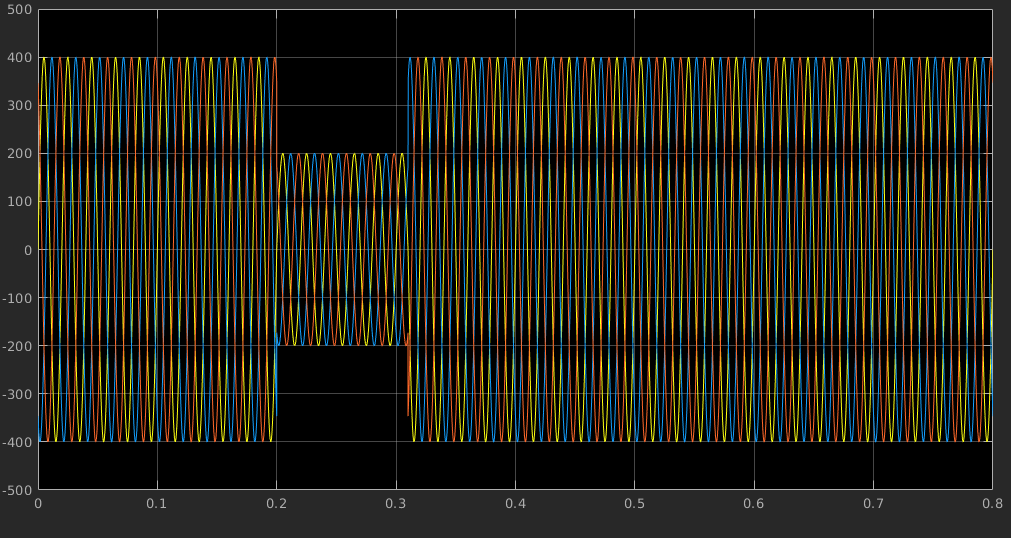
\includegraphics[width=.9\linewidth]{Images/gridvoltageabc.png}
  \caption{Grid voltage in abc components}
  \label{GridV_abc}
\end{figure}

\begin{figure}[H]
  \centering
  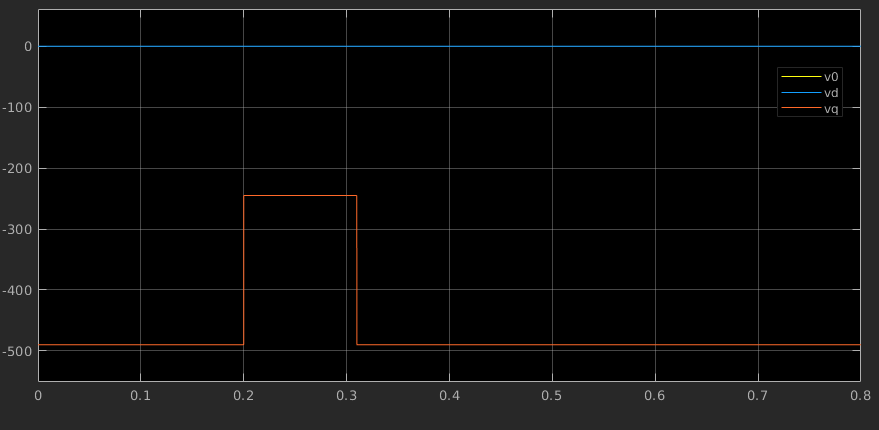
\includegraphics[width=.9\linewidth]{Images/gridvoltagedq.png}
  \caption{Grid voltage in dq components}
  \label{GridV_abc}
\end{figure}

\section{Inverter’s output voltages (phase voltages and line voltages)}

\begin{figure}[H]
  \centering
  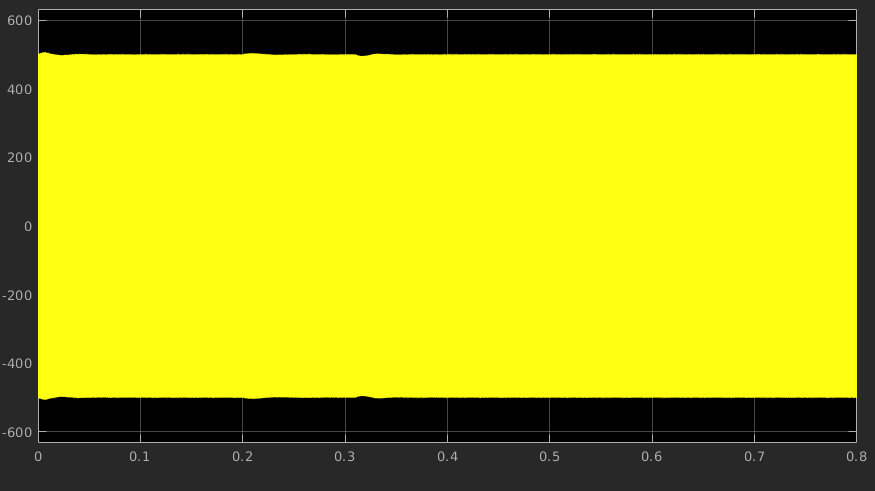
\includegraphics[width=.9\linewidth]{Images/Converter_V_Converter.png}
  \caption{Voltages on the output of the converter}
  \label{ConverterV_abc}
\end{figure}

\begin{figure}[H]
  \centering
  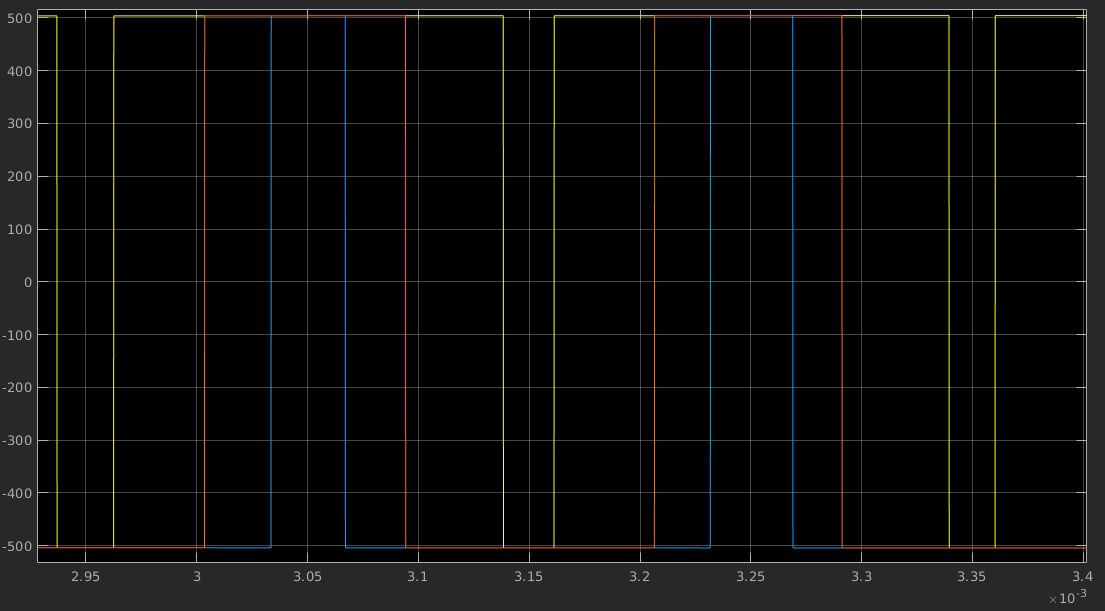
\includegraphics[width=.9\linewidth]{Images/Converter_V_Converter_Zoom.png}
  \caption{Voltages on the output of the converter, zoomed in}
  \label{ConverterV_abc_Zoom}
\end{figure}

\section{DC-link voltage}

\begin{figure}[H]
  \centering
  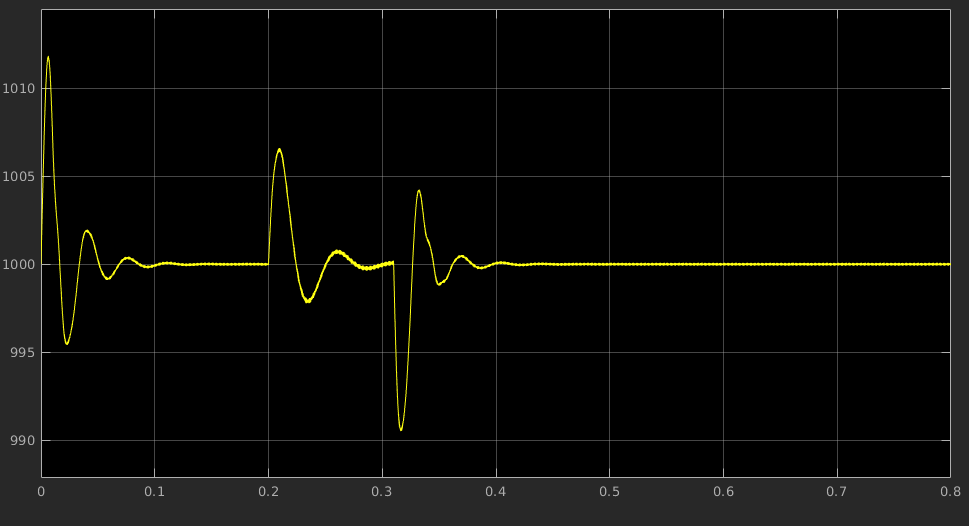
\includegraphics[width=.9\linewidth]{Images/DClink.png}
  \caption{DC link voltage}
  \label{DClink}
\end{figure}

\section{Reference voltages given to the PWM}

\begin{figure}[H]
  \centering
  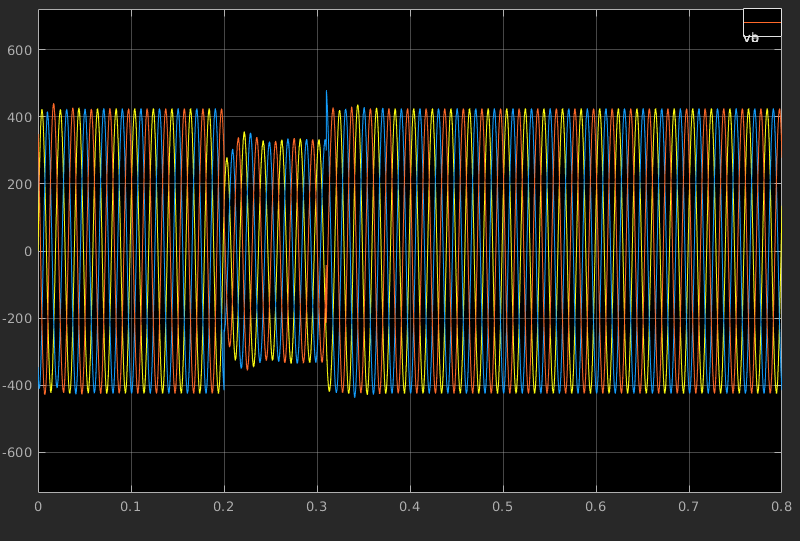
\includegraphics[width=.85\linewidth]{Images/VoltagePWMreference.png}
  \caption{Reference voltages given to the PWM in abc components}
  \label{VoltagePWMreference}
\end{figure}

\begin{figure}[H]
  \centering
  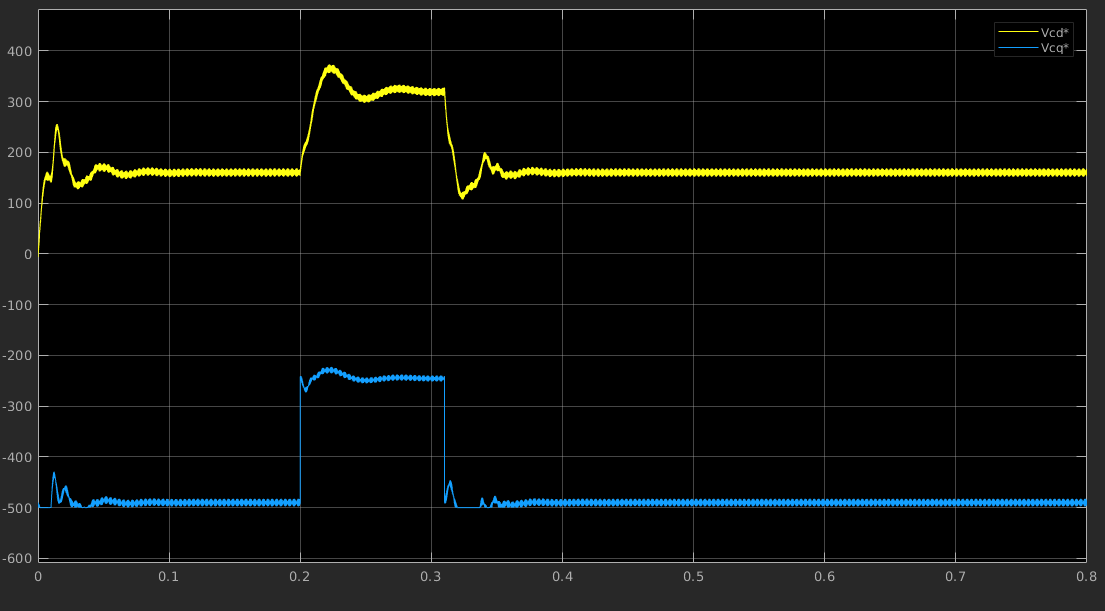
\includegraphics[width=.9\linewidth]{Images/InverterControl_VoltageControl.png}
  \caption{Reference voltages given to the PWM in dq components}
  \label{VoltagePWMreferenceDQ}
\end{figure}

\section{Currents injected by the inverter to the grid (phase abc components and dq components)}

\begin{figure}[H]
  \centering
  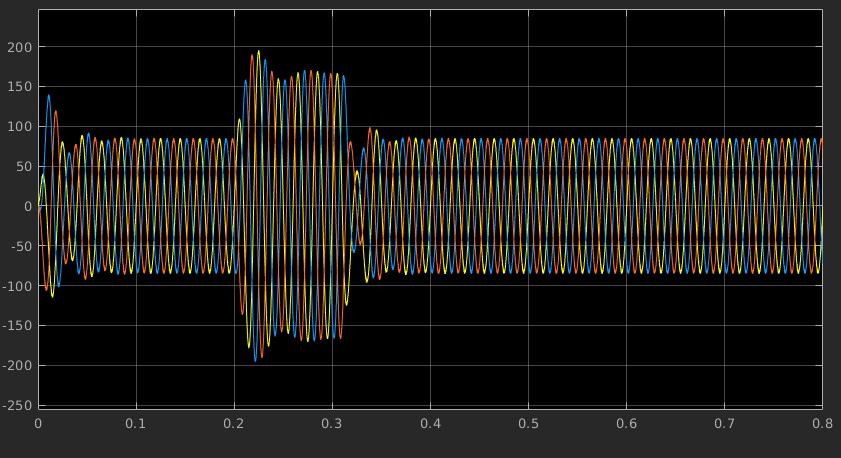
\includegraphics[width=.9\linewidth]{Images/I_filter.png}
  \caption{Currents injected by the inverter to the grid in abc components}
  \label{Currents injected}
\end{figure}

\begin{figure}[H]
  \centering
  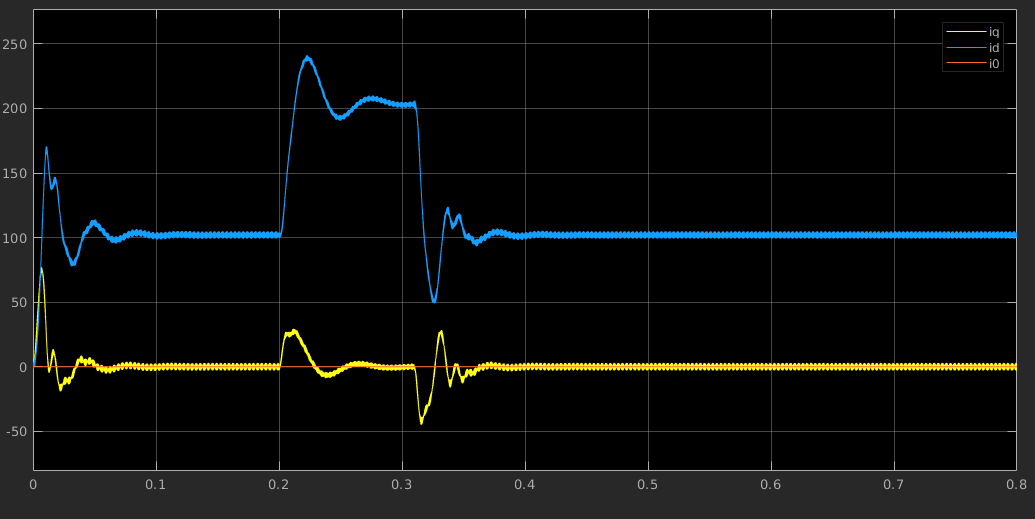
\includegraphics[width=.9\linewidth]{Images/CurrentsParksTransform.png}
  \caption{Currents injected by the inverter to the grid in dq components}
  \label{Currents injected DQ}
\end{figure}

\section{Active power and reactive power delivered to the grid by the inverter}

\begin{figure}[H]
  \centering
  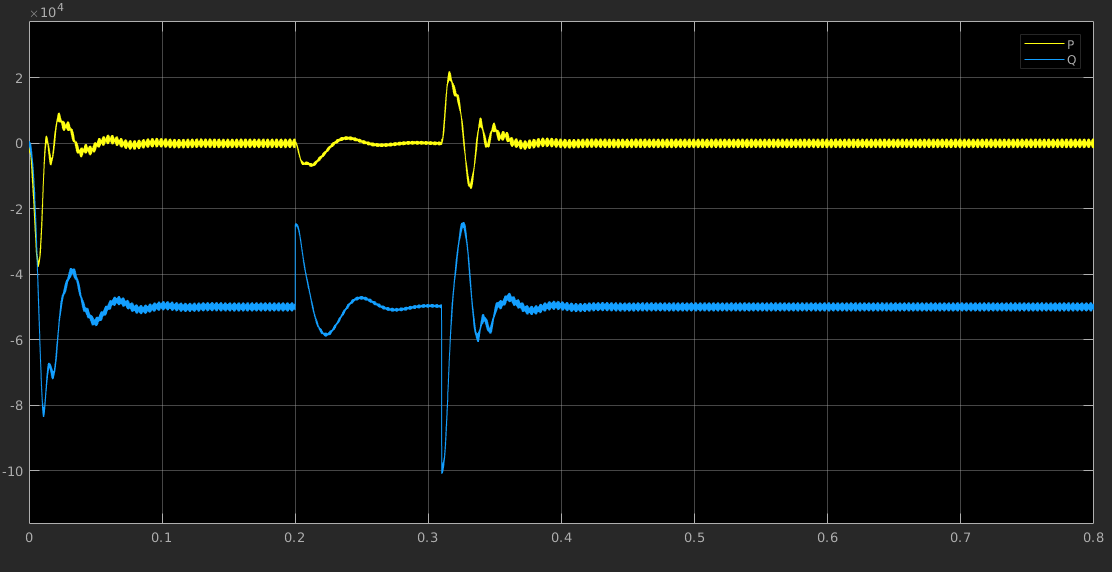
\includegraphics[width=.9\linewidth]{Images/Power.png}
  \caption{Active power and reactive power delivered to the grid by the inverter}
  \label{PowerDelivered}
\end{figure}
